\section{Schaltkreise}

\vspace{1\baselineskip}

\fat{Kirchhoff'sche Regeln}

\begin{tcolorbox}
    \begin{enumerate}
        \item Für jedes aus Widerständen bestehende Schaltelement gilt das \textbf{Ohm'sche Gesetz}: \begin{equation*}
            V_i = R_i I_i
        \end{equation*}
        
        \item Es dürfen sich keine Ladungen aufbauen, daher gilt \begin{equation*}
            \sum_i I_i = 0
            \quad \quad \text{   resp.  } \quad \quad
            \sum I_{\text{in}} =  \sum I_{\text{out}}
        \end{equation*}
        
        \item Für jede Schleife verschwindet die Summe der Potentialdifferenzen: \begin{equation*}
            \sum_i V_i = 0
        \end{equation*}
    \end{enumerate}
\end{tcolorbox}

\vspace{1\baselineskip}

\fat{Ersatzwiderstände}:
\begin{itemize}
    \item Serieschaltung: $R_{\text{Tot}} = \sum_i R_i$
    \item Parallelschaltung: $\frac{1}{R_{\text{Tot}}} = \sum_i \frac{1}{R_i}$
\end{itemize}

\fat{Ersatzkapazitäten}:
\begin{itemize}
    \item Serieschaltung: $\frac{1}{C} = \sum_i \frac{1}{C_i}$
    \item Parallelschaltung: $C = \sum_i C_i$
\end{itemize}

\vspace{1\baselineskip}

\fat{Energieumwandlung}:

Damit eine Ladung durch einen Schaltkreis fliessen kann, muss eine Energiequelle existieren,
welche die in den Widerständen verlorene Wärme ersetzt. Diese Energiequelle wird auch als
\fat{elektromotorische Kraft} $\mathcal{E}$ bezeichnet.

\pagebreak

\fat{Leistung}:
\begin{align*}
    P = \dot{W} = I U = I^2 R = \frac{V^2}{R}
\end{align*}

\vspace{1\baselineskip}

\fat{Schaltkreise mit Kondensatoren}

Es gilt: $Q = C \cdot V$, wobei $Q$ die Ladung, $C$ die Kapazität und $V$ die Spannung ist.

\vspace{1\baselineskip}

\fat{Entladestrom eines Kondensators}:
\begin{align*}
    I(t) = - \frac{V_0}{R} e^{-\nicefrac{t}{R C}}
\end{align*}
Man nennt $R C$ die \fat{Relaxationsskala}.
Der \fat{Ladestrom} ist analog definiert:
\begin{align*}
    I(t) = \frac{V_0}{R} e^{-\nicefrac{t}{R C}}
\end{align*}

\vspace{1\baselineskip}

\fat{Das Vorzeichen ABC}

\vspace{1\baselineskip}

\begin{minipage}{0.25\textwidth}
    \begin{center}
        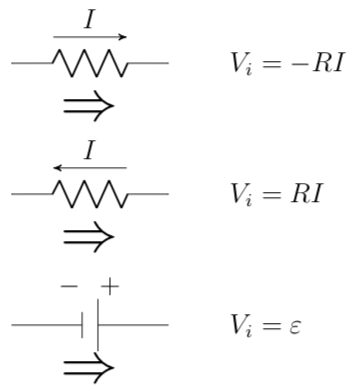
\includegraphics[width=0.8\textwidth]{Figures/Vorzeichen1.png}
    \end{center}
\end{minipage}
\begin{minipage}{0.25\textwidth}
    \begin{center}    
        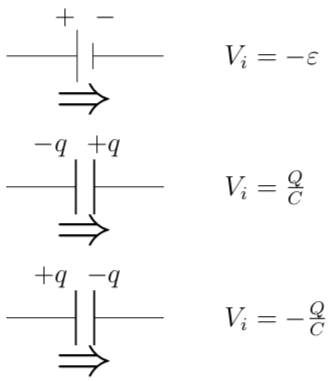
\includegraphics[width=0.8\textwidth]{Figures/Vorzeichen2.png}
    \end{center}
\end{minipage}
